\documentclass{article}\usepackage[]{graphicx}\usepackage[]{color}
%% maxwidth is the original width if it is less than linewidth
%% otherwise use linewidth (to make sure the graphics do not exceed the margin)
\makeatletter
\def\maxwidth{ %
  \ifdim\Gin@nat@width>\linewidth
    \linewidth
  \else
    \Gin@nat@width
  \fi
}
\makeatother

\usepackage{Sweavel}



\usepackage{amsmath}
\usepackage[affil-it]{authblk}
\usepackage{hyperref}

\usepackage{listings} % to add code line break
\lstset{breaklines=true,showstringspaces=false}


\begin{document}


\title{Reproducing Scott's Paper}
\author{Kejun He}
\affil{Department of Statistics,\\ Texas A\&M University}

\maketitle

\tableofcontents

\section{Metabolic}
 \subsection{Oct 8}
   Reproducing and rearrangeing  \textit{metabolic\_\ignorespaces analysis\_\ignorespaces script.txt}
   \begin{center}
\begin{Schunk}


{\centering 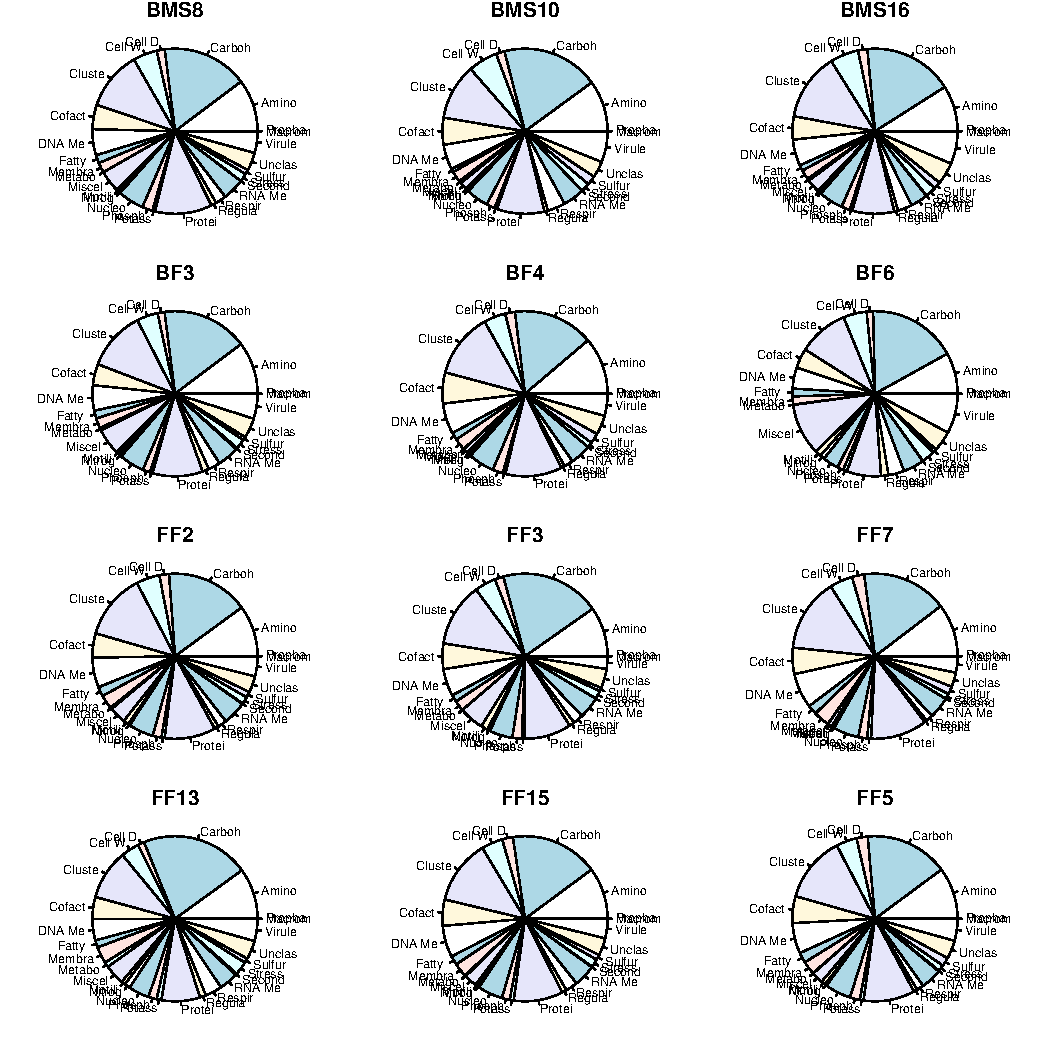
\includegraphics[width=\maxwidth]{figure/Oct_8-1} 

}

\end{Schunk}
   \end{center}
   The piecharts above show the proportion of each SEEDlevel1 in each individual. 
  $ $
  \newpage
  
  \subsection{Oct 9}
  % Reproducing and rearrangeing  \textit{metabolic\_\ignorespaces analysis\_\ignorespaces script.txt}
   %\vfill
   \begin{center}
\begin{Schunk}


{\centering 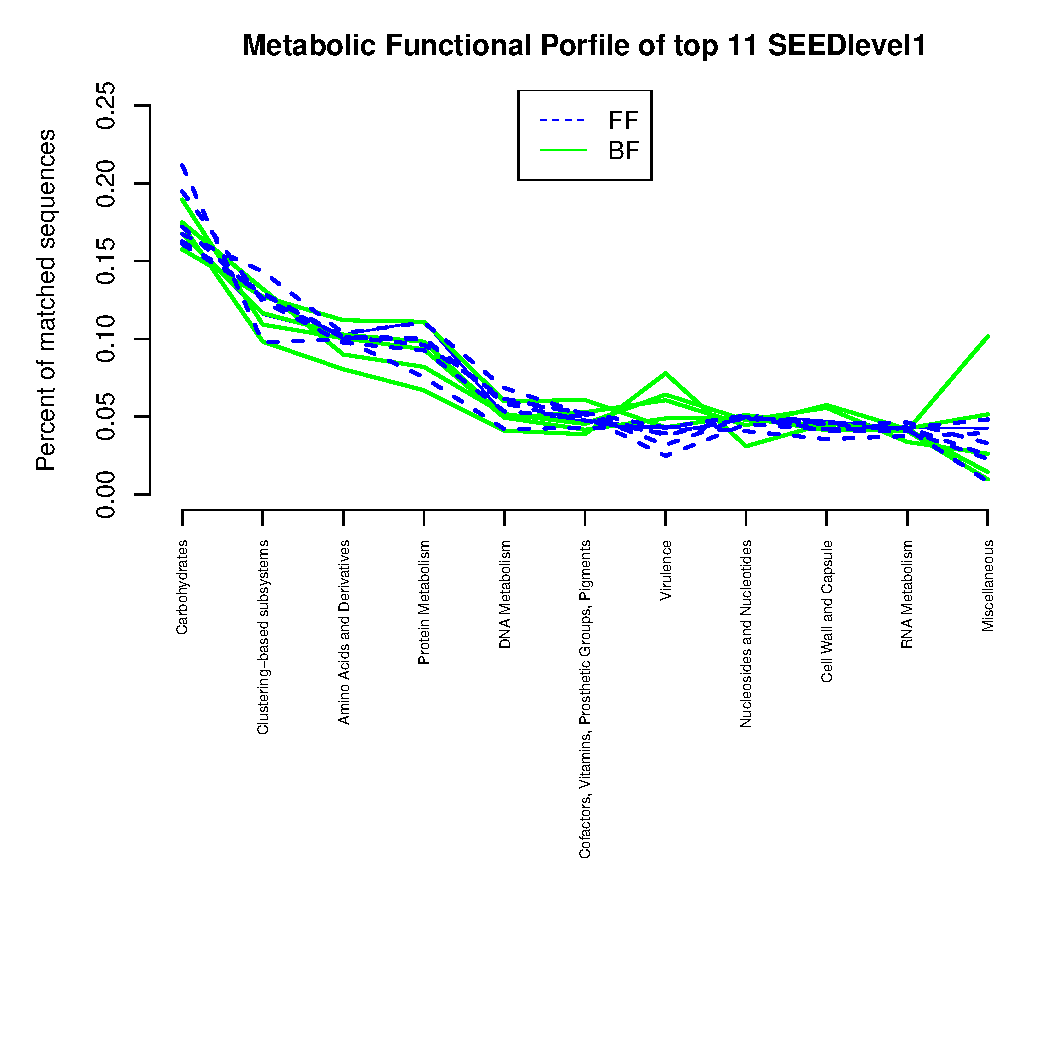
\includegraphics[width=\maxwidth]{figure/Oct_9-1} 

}



{\centering 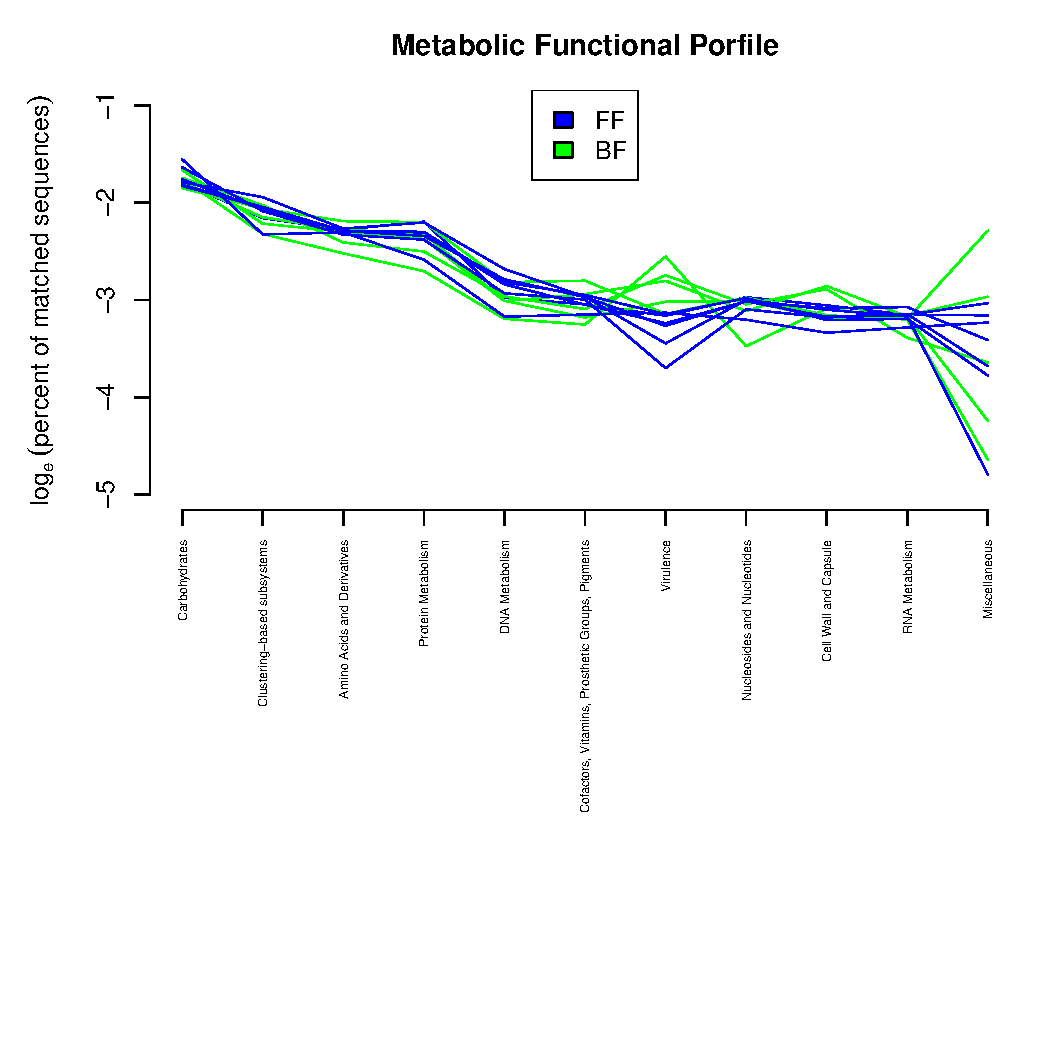
\includegraphics[width=\maxwidth]{figure/Oct_9-2} 

}



{\centering 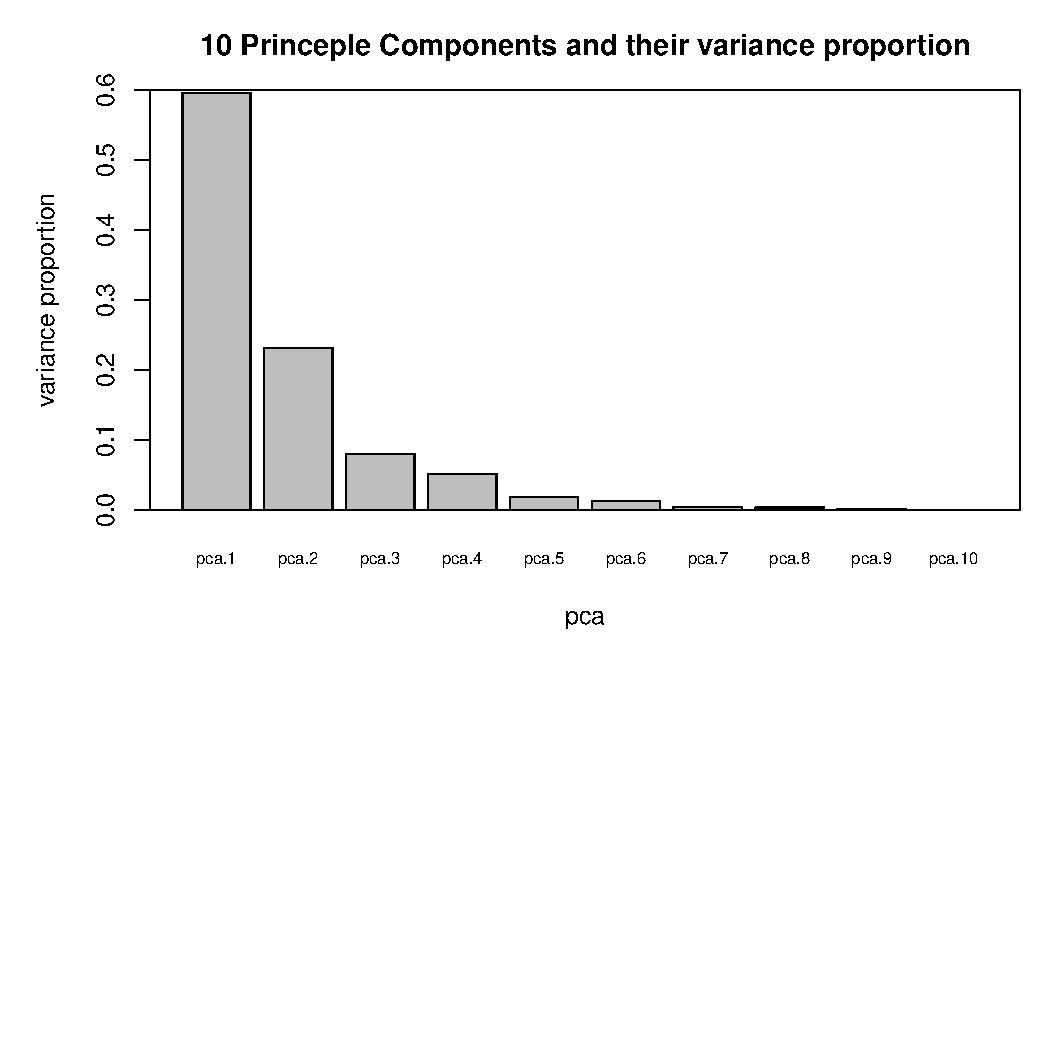
\includegraphics[width=\maxwidth]{figure/Oct_9-3} 

}



{\centering 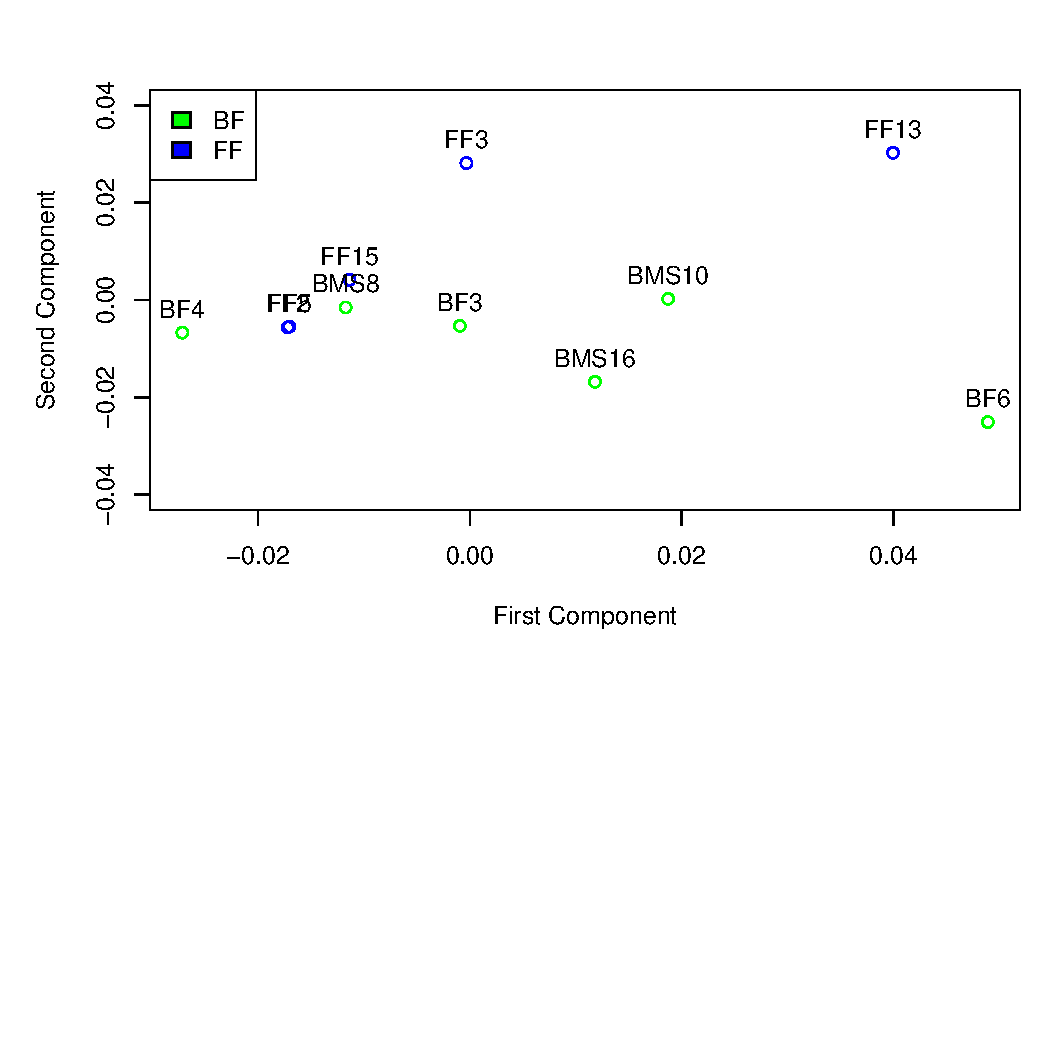
\includegraphics[width=\maxwidth]{figure/Oct_9-4} 

}

\end{Schunk}
   \end{center}

  \subsection{Oct 10}
   Reproducing and rearrangeing \textit{metabolic\_\ignorespaces analysis\_\ignorespaces script.txt}
   \begin{center}
\begin{Schunk}


{\centering 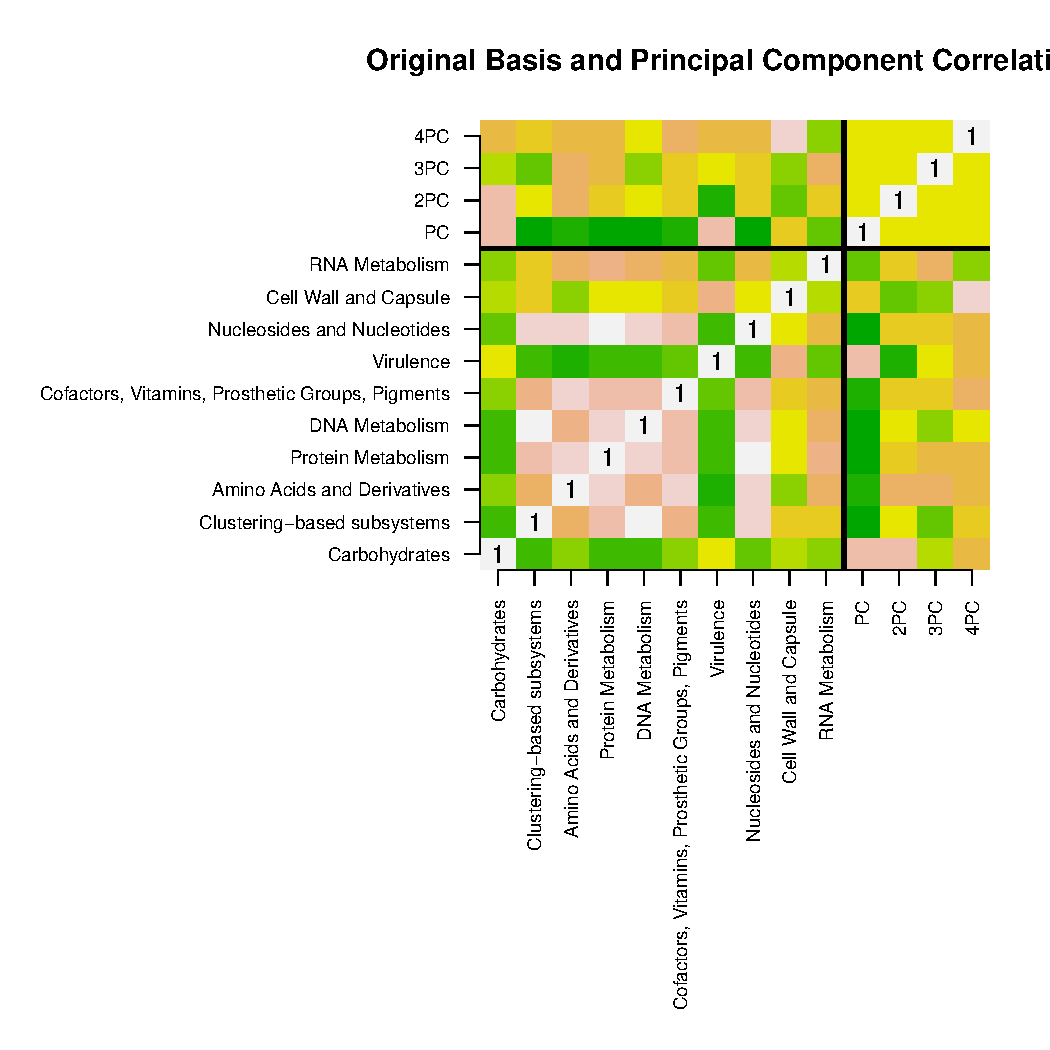
\includegraphics[width=\maxwidth]{figure/oct_10-1} 

}



{\centering 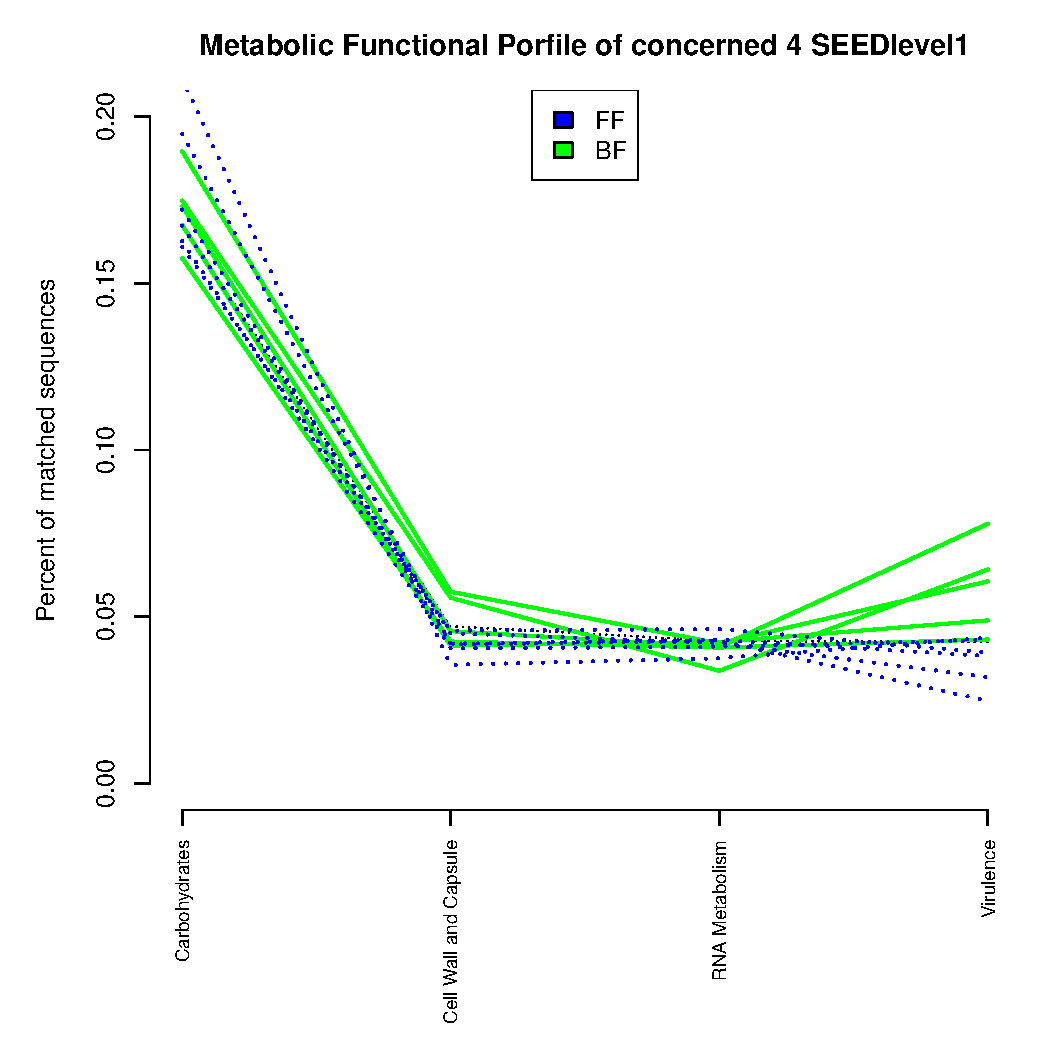
\includegraphics[width=\maxwidth]{figure/oct_10-2} 

}

\end{Schunk}
   \end{center}
   
   
  \subsection{Oct 12}
stop at line 410.
scotts\_\ignorespaces Immunology\_\ignorespaces set is on CCA part (around the end) of ``paper\_\ignorespaces figure\_\ignorespaces analysis.txt''. 

  
\begin{Schunk}


{\centering 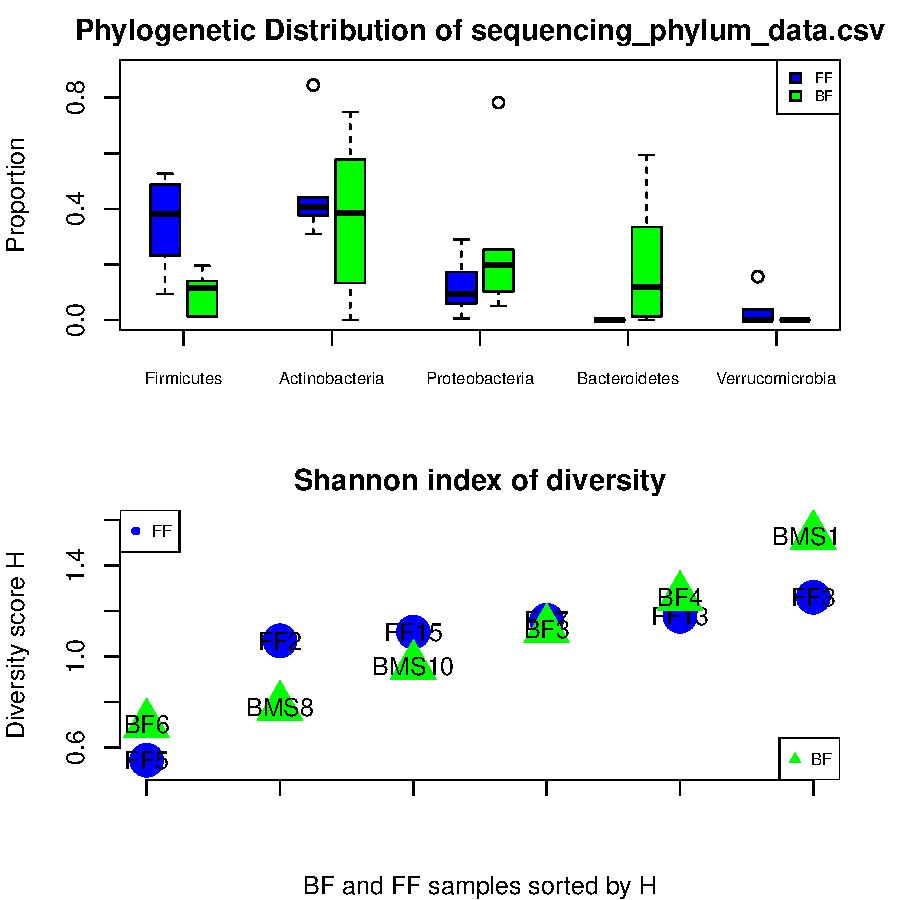
\includegraphics[width=\maxwidth]{figure/Oct_12-1} 

}

\end{Schunk}

  \subsection{Oct 15}
  
\begin{Schunk}


{\centering 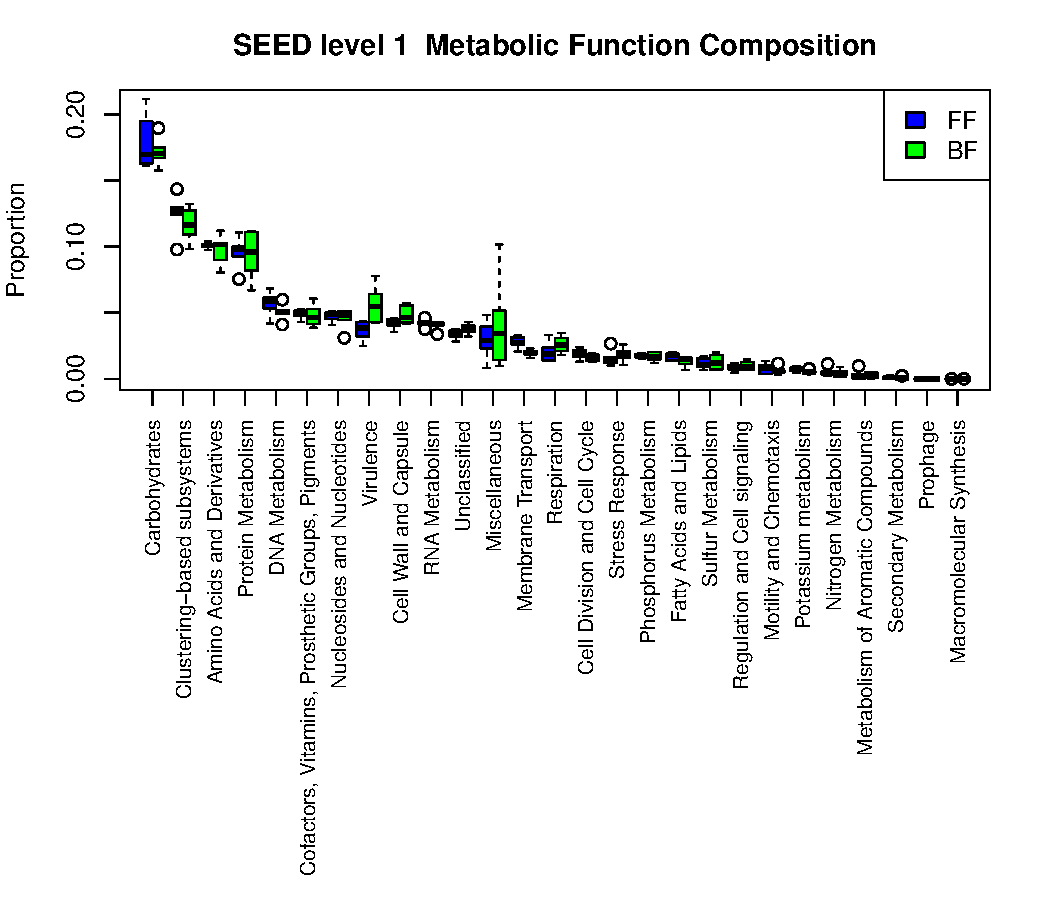
\includegraphics[width=\maxwidth]{figure/Oct_15_1-1} 

}



{\centering 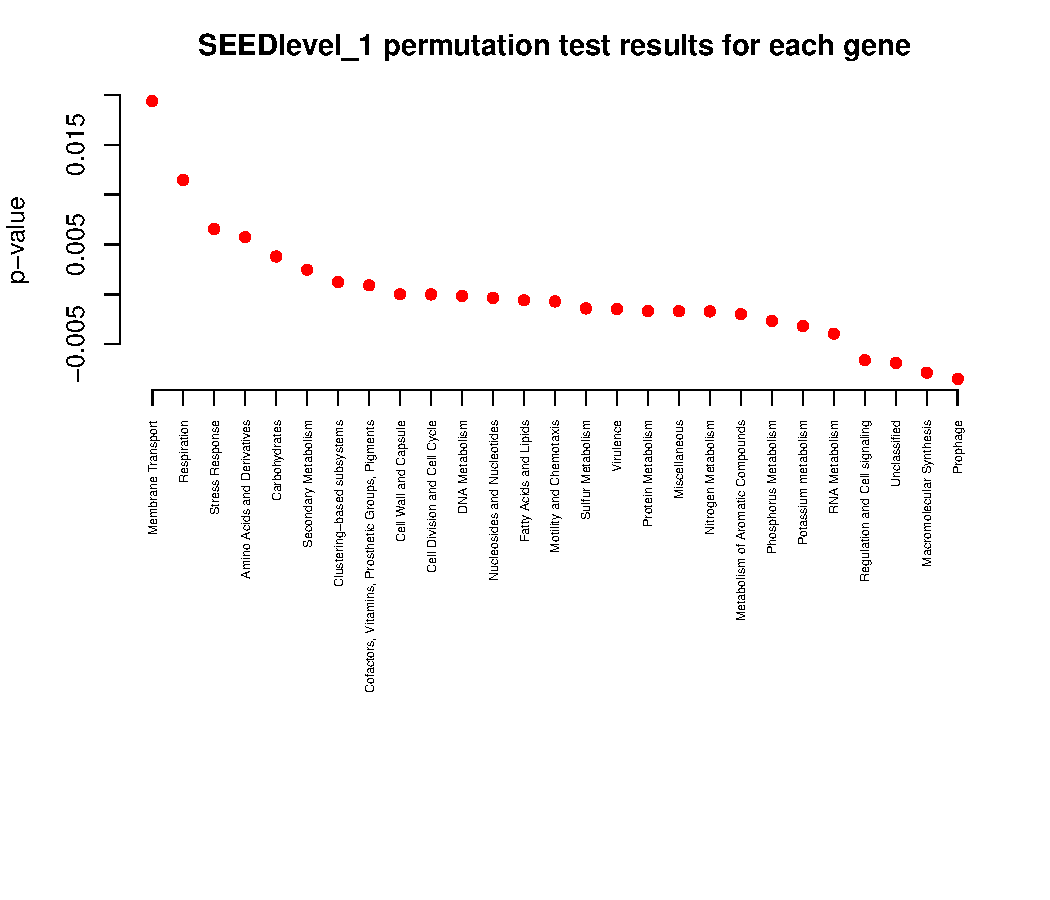
\includegraphics[width=\maxwidth]{figure/Oct_15_1-2} 

}



{\centering 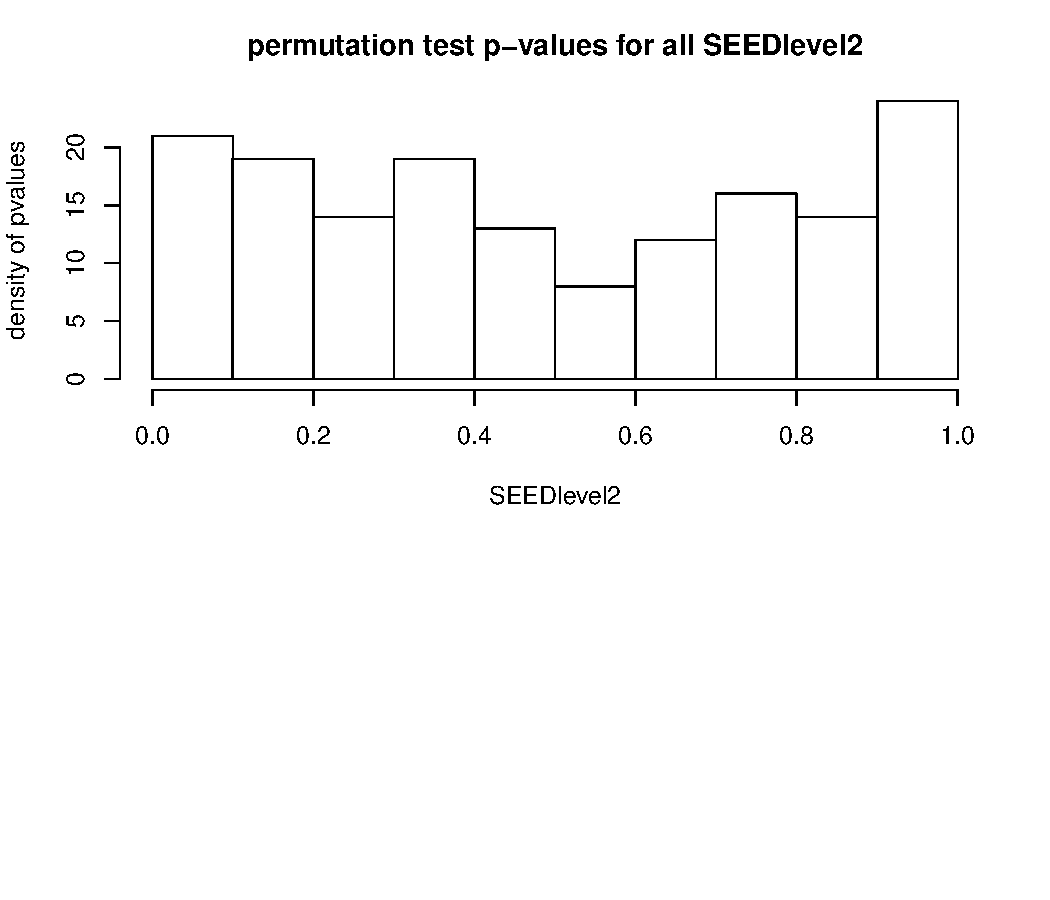
\includegraphics[width=\maxwidth]{figure/Oct_15_1-3} 

}



{\centering 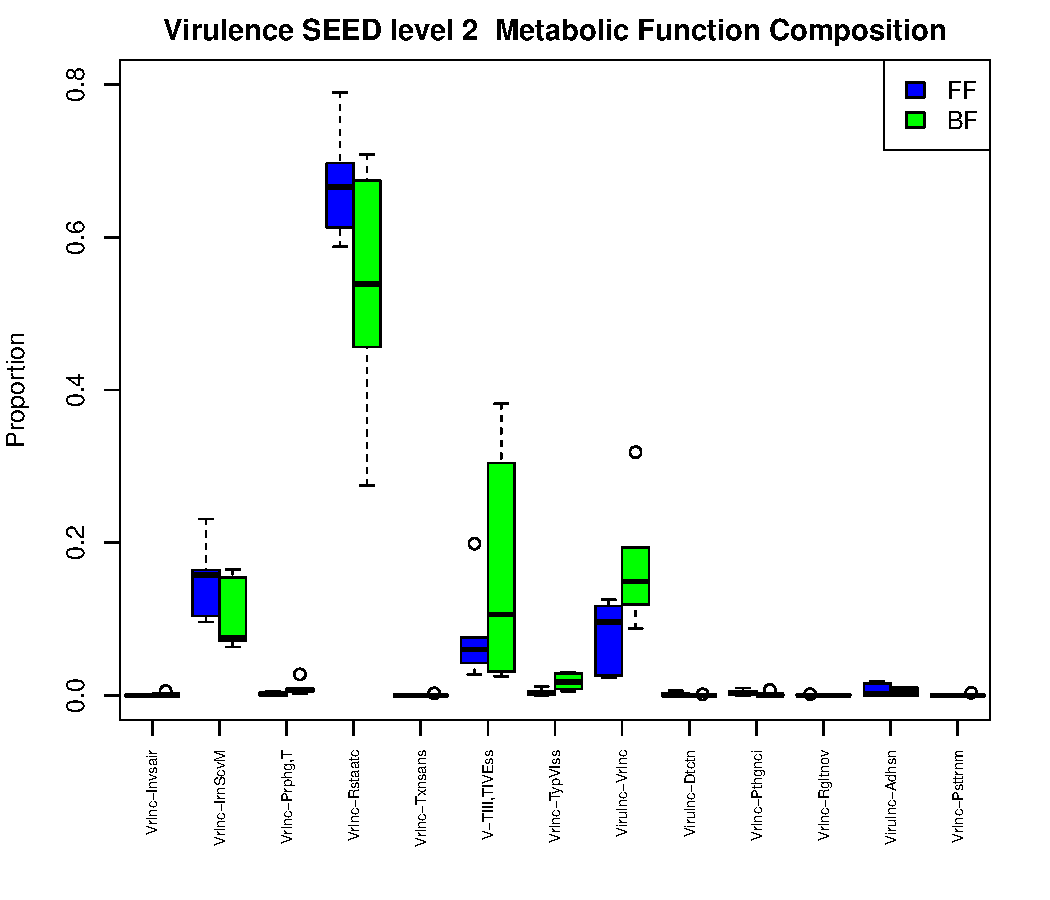
\includegraphics[width=\maxwidth]{figure/Oct_15_1-4} 

}



{\centering 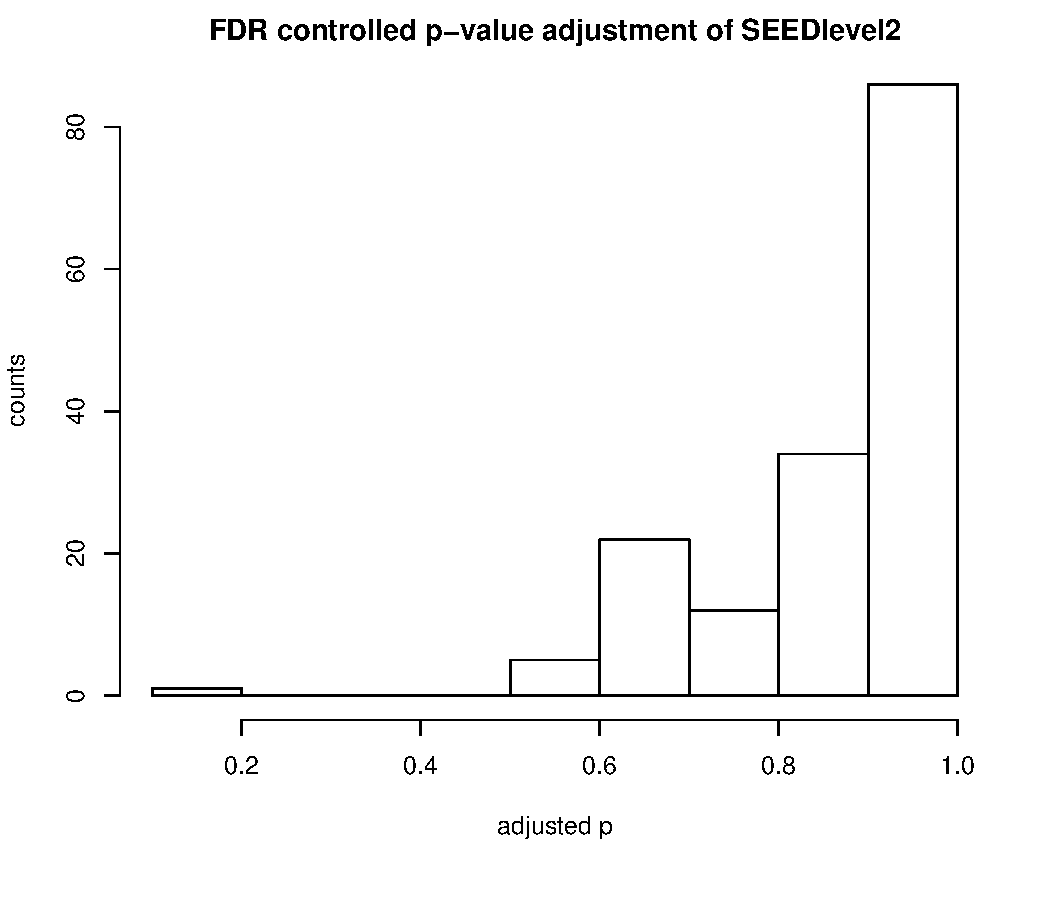
\includegraphics[width=\maxwidth]{figure/Oct_15_1-5} 

}

\end{Schunk}


  \subsection{Oct 19}
   Seedlevel3
\begin{Schunk}


{\centering 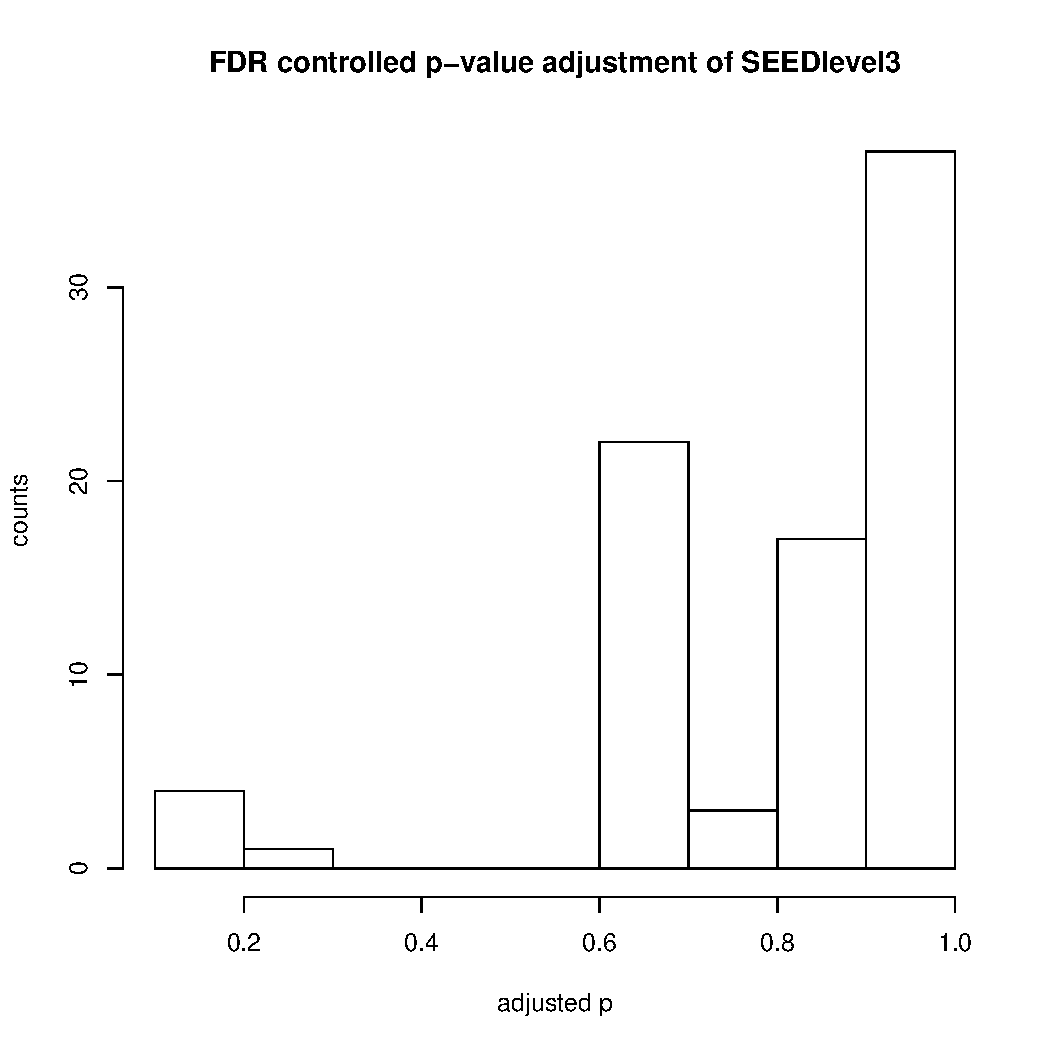
\includegraphics[width=\maxwidth]{figure/Oct_19_Seed-1} 

}

\end{Schunk}


\section{Microarray}

  \subsection{Oct 23 \& Oct 25}
\begin{Schunk}


{\centering 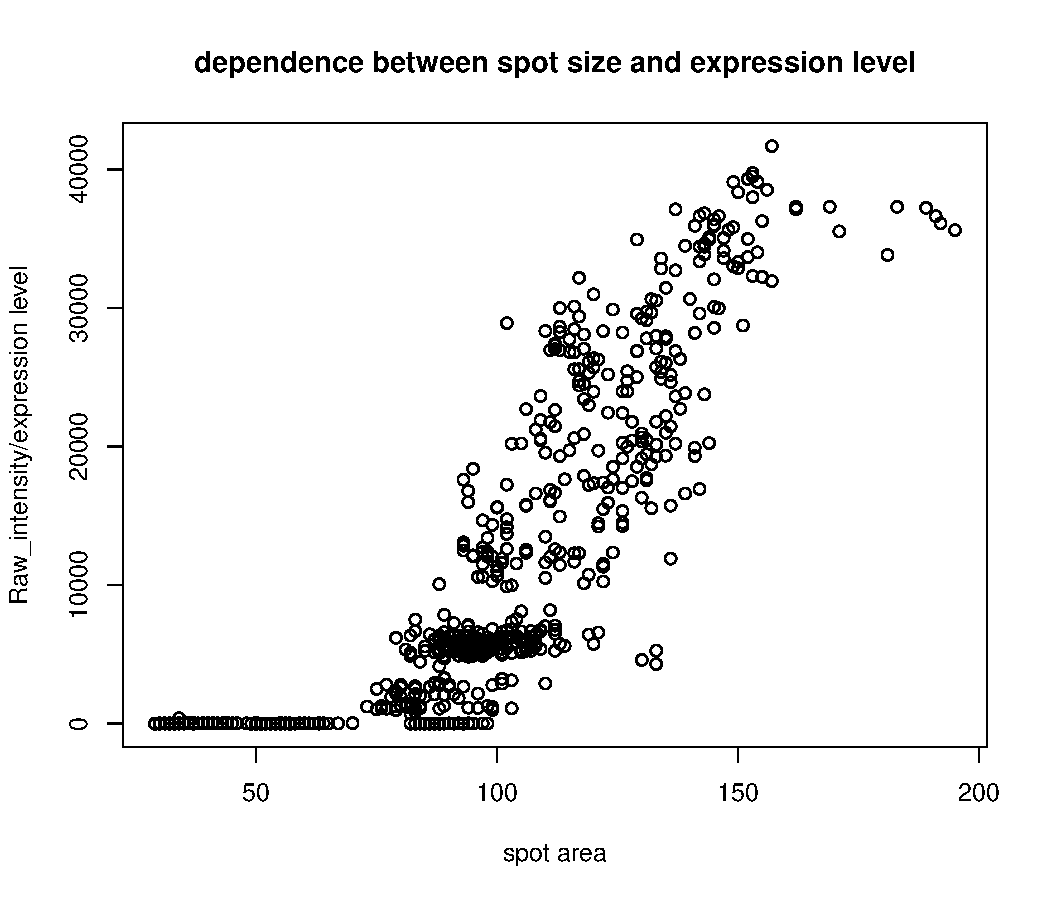
\includegraphics[width=\maxwidth]{figure/Oct_23_start_micro-1} 

}

\end{Schunk}


  \subsection{Nov 3}
  
\begin{Schunk}


{\centering 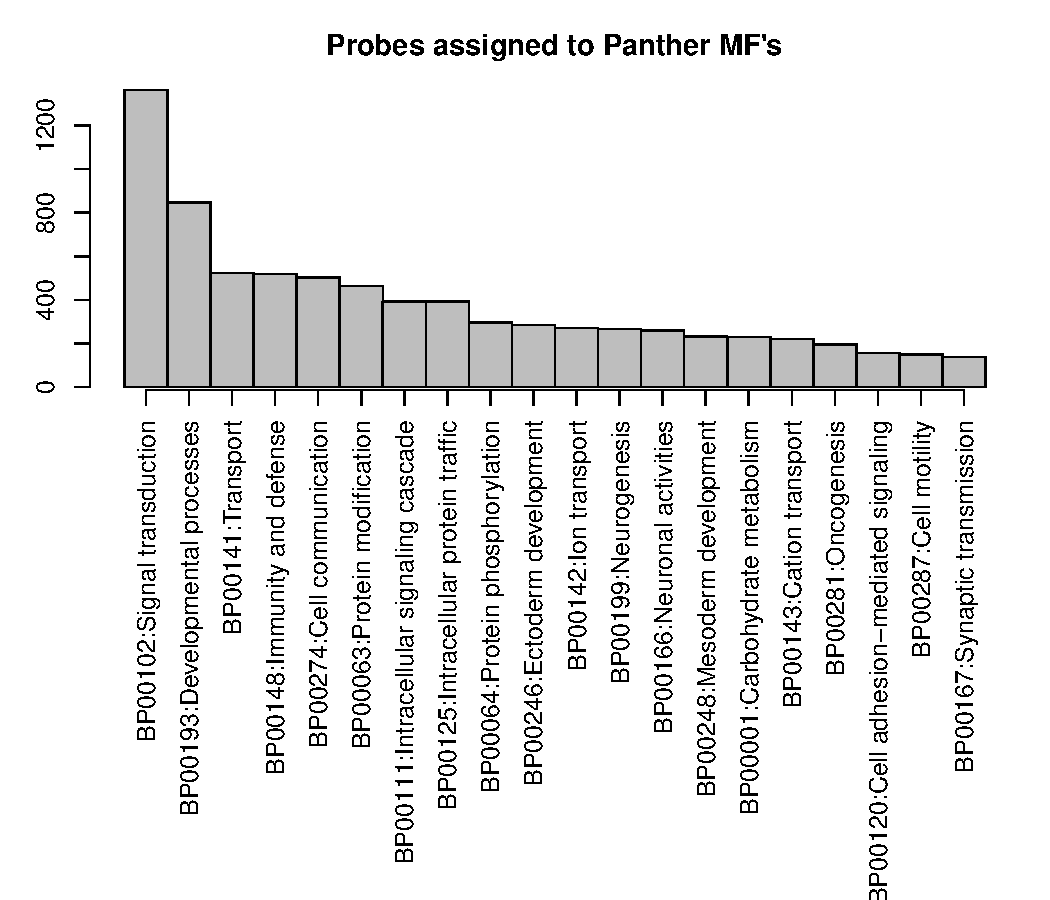
\includegraphics[width=\maxwidth]{figure/Nov_3_gene_list_and_testing-1} 

}



{\centering 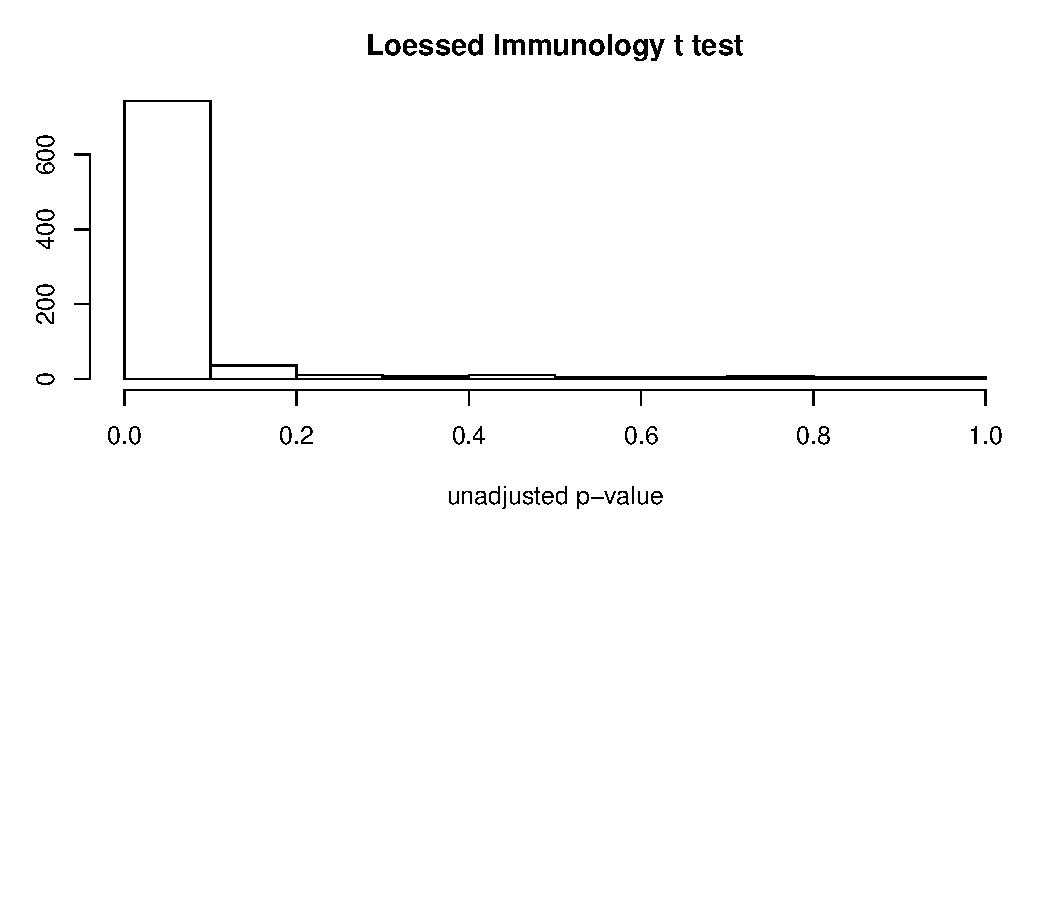
\includegraphics[width=\maxwidth]{figure/Nov_3_gene_list_and_testing-2} 

}



{\centering 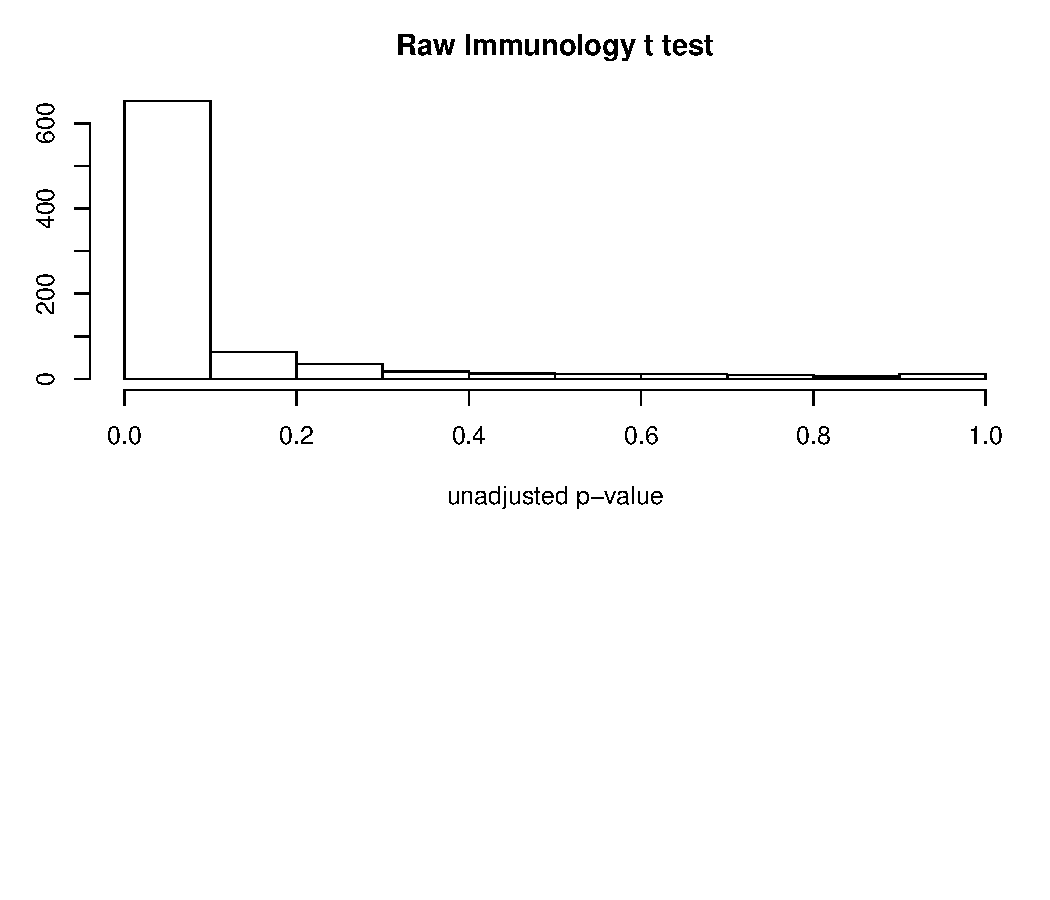
\includegraphics[width=\maxwidth]{figure/Nov_3_gene_list_and_testing-3} 

}

\end{Schunk}

  \subsection{Nov 5}
  After getting the Intestinal gene data.
\begin{Schunk}


{\centering 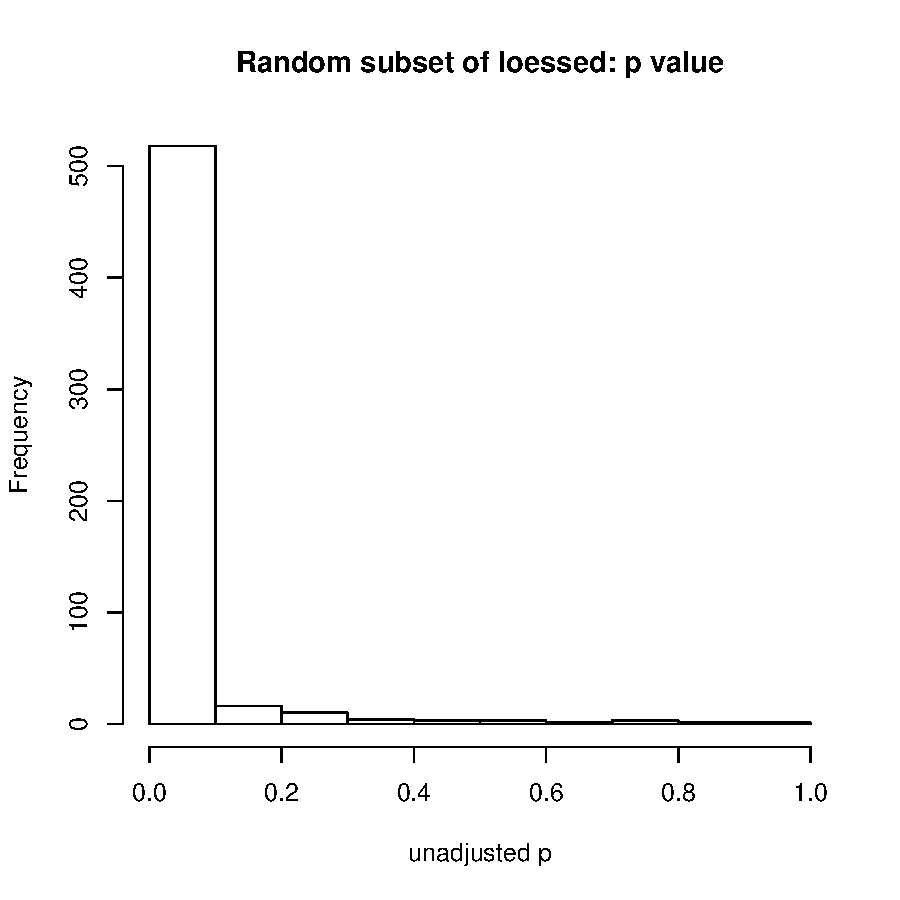
\includegraphics[width=\maxwidth]{figure/Nov_5-1} 

}



{\centering 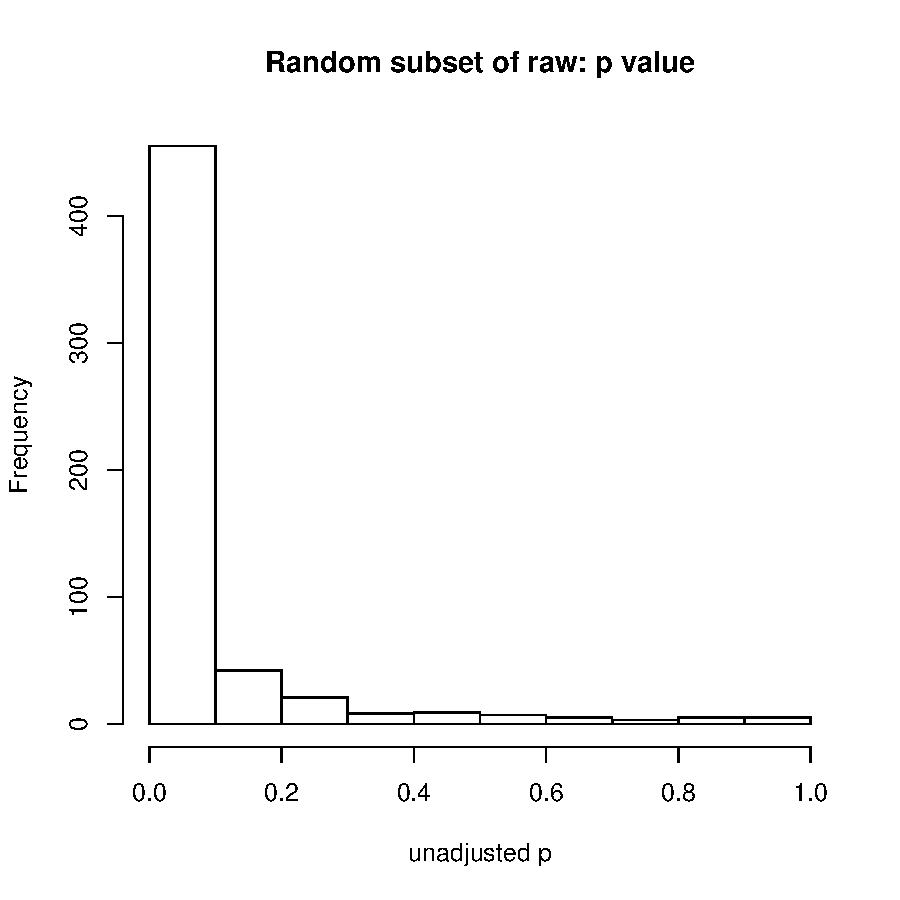
\includegraphics[width=\maxwidth]{figure/Nov_5-2} 

}

\end{Schunk}

  \subsection{Nov 9}
\begin{Schunk}

\begin{Soutput}
Call: CCA.permute(x = cca_seed2_BF, z = cca_microarray_subjects_BF, 
    typex = "standard", typez = "standard", nperms = 7)

Type of x:  standard 
Type of z:  standard 
   X Penalty Z Penalty Z-Stat P-Value  Cors Cors Perm
1      0.100     0.100 -0.015   0.429 0.995     0.994
2      0.167     0.167  0.850   0.286 0.997     0.993
3      0.233     0.233  2.465   0.000 0.998     0.992
4      0.300     0.300  1.422   0.143 0.996     0.990
5      0.367     0.367  0.152   0.143 0.991     0.987
6      0.433     0.433 -0.161   0.286 0.984     0.983
7      0.500     0.500 -0.180   0.571 0.977     0.976
8      0.567     0.567 -0.145   0.571 0.971     0.970
9      0.633     0.633 -0.205   0.571 0.967     0.966
10     0.700     0.700 -0.293   0.571 0.963     0.965
   FT(Cors) FT(Cors Perm) # U's Non-Zero # Vs Non-Zero
1     2.978         2.983              4             9
2     3.311         2.941              7            26
3     3.501         2.790             10            59
4     3.134         2.688             18            89
5     2.713         2.643             24           131
6     2.404         2.474             34           178
7     2.216         2.286             42           234
8     2.106         2.157             55           305
9     2.037         2.117             70           374
10    1.988         2.113             95           458
Best L1 bound for x:  0.2333333
Best L1 bound for z:  0.2333333
\end{Soutput}


{\centering 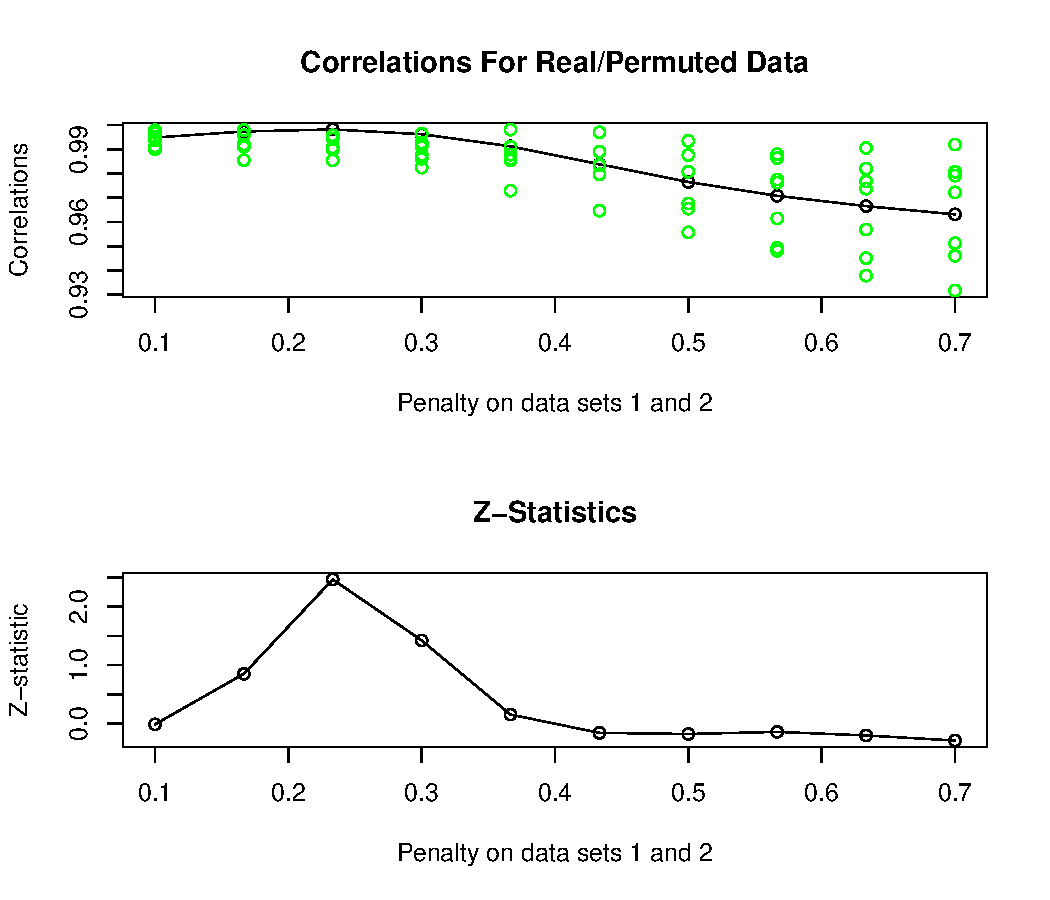
\includegraphics[width=\maxwidth]{figure/Nov_9-1} 

}

\begin{Soutput}
123456789101112131415
\end{Soutput}
\begin{Soutput}
Call: CCA(x = cca_seed2_BF, z = cca_microarray_subjects_BF, typex = "standard", 
    typez = "standard", penaltyx = 0.2333, penaltyz = 0.2333, 
    xnames = abbreviate(colnames(cca_seed2_BF), min = 20), znames = colnames(cca_microarray_subjects_BF))


Num non-zeros u's:  10 
Num non-zeros v's:  56 
Type of x:  standard 
Type of z:  standard 
Penalty for x: L1 bound is  0.2333 
Penalty for z: L1 bound is  0.2333 
Cor(Xu,Zv):  0.9991598

 Component  1 :

   Row Feature Name     Row Feature Weight
1  Rsprtn-Elctrnaccptnr 0.115             
2  Crbhydrts-Clstrng-bs 0.462             
3  Clstrng-bs-DNApIIIec 0.166             
4  Clstrng-bsdsbs-TldDc 0.338             
5  DNAMtblsm-DNAuptk,cm 0.518             
6  SlfrMtblsm-Orgncslfa 0.158             
7  Vrln-TIII,TIV,ESATss 0.367             
8  Vrlnc-TypVIscrtnsyst 0.358             
9  ProtnMtblsm-Slnprtns 0.17              
10 Miscellaneos-Mscllns 0.215             

   Column Feature Name Column Feature Weight
1  PLAU                -0.086               
2  HLA-E               -0.047               
3  IL1B                -0.2                 
4  TBX21               -0.042               
5  MSRA                -0.064               
6  OASL                -0.035               
7  CXCL2               -0.014               
8  ARHGAP9             -0.077               
9  HSH2D               -0.158               
10 RGS1                -0.08                
11 IRF7                -0.138               
12 NFKBIA              -0.234               
13 TYROBP              -0.17                
14 HLA-G               -0.049               
15 CASP1               -0.271               
16 STAT5B              -0.066               
17 SLA                 -0.046               
18 SOD2                -0.044               
19 ABCB10              -0.032               
20 MAPKAPK2            -0.053               
21 NR4A3               -0.078               
22 IFITM1              -0.224               
23 EIF2AK2             -0.113               
24 FZD1                0.185                
25 ICAM3               -0.164               
26 IL11RA              -0.001               
27 CLEC4F              -0.206               
28 ARHGAP23            -0.054               
29 IL8                 -0.248               
30 TFCP2               -0.109               
31 HLA-DMA             0.002                
32 THBS4               -0.155               
33 TICAM1              -0.03                
34 SEMA4D              -0.137               
35 IFI30               -0.212               
36 IFITM2              -0.079               
37 ICAM3               -0.028               
38 IER3                -0.146               
39 ITPR1               0.207                
40 GSTM3               -0.159               
41 GPX1                -0.003               
42 ISG20               -0.087               
43 IRAK1               -0.002               
44 HLA-F               -0.12                
45 MMP9                -0.244               
46 CXCL16              -0.044               
47 ARHGAP30            0.031                
48 SOD2                -0.186               
49 F13B                0.04                 
50 IL7R                0.061                
51 NFKB1               -0.211               
52 THBS1               -0.143               
53 CD200               -0.163               
54 NUP88               -0.007               
55 WAS                 -0.242               
56 S100A8              -0.076               
\end{Soutput}

\begin{Soutput}
Call: CCA.permute(x = cca_seed2_FF, z = cca_microarray_subjects_FF, 
    typex = "standard", typez = "standard", nperms = 7)

Type of x:  standard 
Type of z:  standard 
   X Penalty Z Penalty Z-Stat P-Value  Cors Cors Perm
1      0.100     0.100 -1.336   1.000 0.957     0.986
2      0.167     0.167 -1.796   1.000 0.960     0.986
3      0.233     0.233 -1.046   0.857 0.967     0.981
4      0.300     0.300  0.130   0.429 0.978     0.974
5      0.367     0.367  0.862   0.143 0.981     0.962
6      0.433     0.433  1.580   0.000 0.981     0.950
7      0.500     0.500  1.777   0.000 0.975     0.937
8      0.567     0.567  1.776   0.000 0.970     0.932
9      0.633     0.633  0.955   0.143 0.965     0.933
10     0.700     0.700  0.473   0.143 0.958     0.931
   FT(Cors) FT(Cors Perm) # U's Non-Zero # Vs Non-Zero
1     1.912         2.629              4            10
2     1.951         2.511              6            25
3     2.051         2.391             13            54
4     2.242         2.208             18            94
5     2.336         2.031             24           140
6     2.312         1.869             36           198
7     2.185         1.744             46           267
8     2.090         1.695             57           349
9     2.009         1.725             68           435
10    1.916         1.739             87           526
Best L1 bound for x:  0.5
Best L1 bound for z:  0.5
\end{Soutput}


{\centering 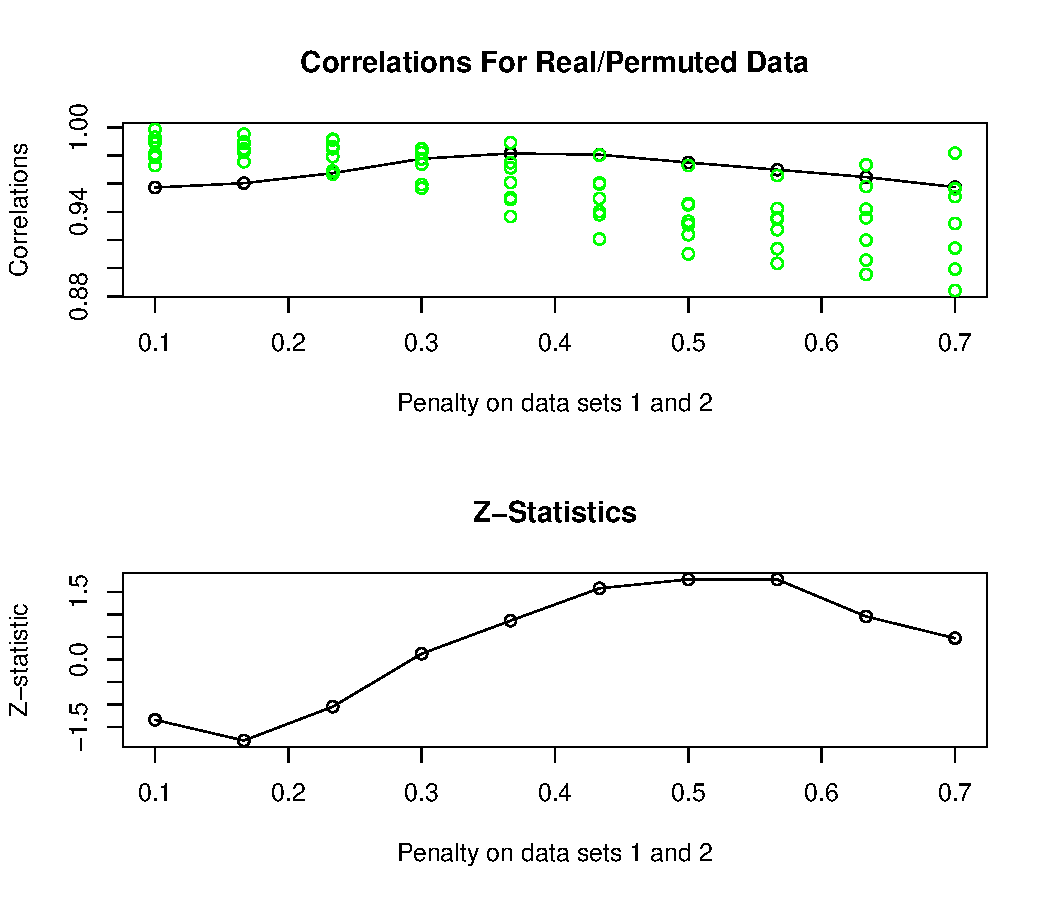
\includegraphics[width=\maxwidth]{figure/Nov_9-2} 

}

\begin{Soutput}
123456789101112131415
\end{Soutput}
\begin{Soutput}
Call: CCA(x = cca_seed2_FF, z = cca_microarray_subjects_FF, typex = "standard", 
    typez = "standard", penaltyx = 0.2333, penaltyz = 0.2333, 
    xnames = abbreviate(colnames(cca_seed2_FF), min = 20), znames = colnames(cca_microarray_subjects_FF))


Num non-zeros u's:  13 
Num non-zeros v's:  55 
Type of x:  standard 
Type of z:  standard 
Penalty for x: L1 bound is  0.2333 
Penalty for z: L1 bound is  0.2333 
Cor(Xu,Zv):  0.9763865

 Component  1 :

   Row Feature Name     Row Feature Weight
1  Crbhydrts-Clstrng-bs -0.024            
2  Crbhydrts-On-crbnMtb -0.514            
3  Carbhydrts-Uptksystm -0.074            
4  Clstrng-bsdsbsy-CoUF -0.256            
5  C-s-D--RNA(T)d(EC3.c -0.049            
6  Clstrng-bsdsbsy-Famc -0.431            
7  Clstrng-bsdsbs-HiLbc -0.362            
8  Clstrng-bsdsbsys-LBc -0.338            
9  Clstrng-s-Lys,t,m,ac -0.156            
10 Clstrng-bsdsbs-TldDc -0.441            
11 CllWllandCpsl-Cpsaep -0.086            
12 CllWllandCp-Grm-Ncwc -0.017            
13 Miscellaneos-Mscllns -0.072            

   Column Feature Name Column Feature Weight
1  IL17B               -0.027               
2  AIM2                -0.052               
3  MAP4K4              -0.005               
4  PRG3                -0.032               
5  LEF1                0.1                  
6  CXCL1               0.094                
7  IKBKAP              -0.053               
8  MOSC1               -0.093               
9  WASL                -0.238               
10 VTN                 0.253                
11 IL6R                -0.058               
12 MMD                 -0.224               
13 NFKBIB              -0.145               
14 C1QTNF6             0.222                
15 COLEC10             0.214                
16 EGFR                -0.088               
17 LPO                 0.261                
18 MALT1               -0.004               
19 PPIL1               -0.06                
20 EIF2AK2             0.163                
21 CASP8               -0.188               
22 C1RL                0.054                
23 PPP3CA              -0.078               
24 C1QL2               -0.217               
25 CXCR3               -0.04                
26 BMPR1A              -0.014               
27 MSRB3               -0.2                 
28 SP3                 -0.179               
29 SEMA4A              0.05                 
30 SMAD5               0.029                
31 PAFAH2              0.058                
32 TACR3               -0.244               
33 ITPR1               -0.181               
34 LTB4R2              -0.033               
35 OAS1                0.164                
36 HRH1                0.034                
37 IL17RD              -0.178               
38 AOC3                -0.153               
39 ULBP2               -0.022               
40 CR2                 0.109                
41 TYRO3               -0.177               
42 CCR7                0.031                
43 ALOX5               -0.095               
44 LTBP4               0.007                
45 CXCL16              0.114                
46 ALOX5               -0.189               
47 TGFB3               -0.02                
48 CCL21               -0.042               
49 FGFR1               0.145                
50 CD40                -0.085               
51 ABCC5               -0.208               
52 PVRL2               0.028                
53 GYPC                -0.089               
54 PTK2B               0.12                 
55 NDST1               -0.146               
\end{Soutput}
\end{Schunk}

 \subsection{Nov 16}
 ggplot the scatterplots of first components
\begin{Schunk}


{\centering 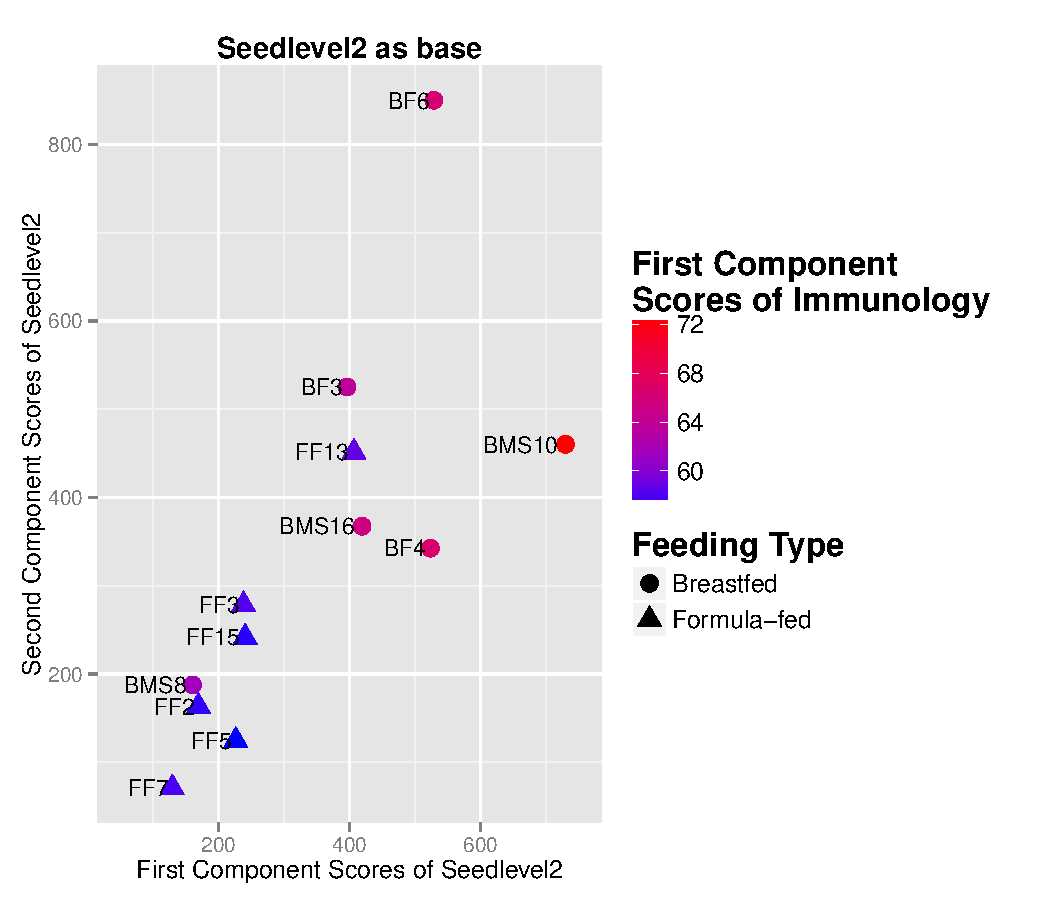
\includegraphics[width=\maxwidth]{figure/Nov_16-1} 

}



{\centering 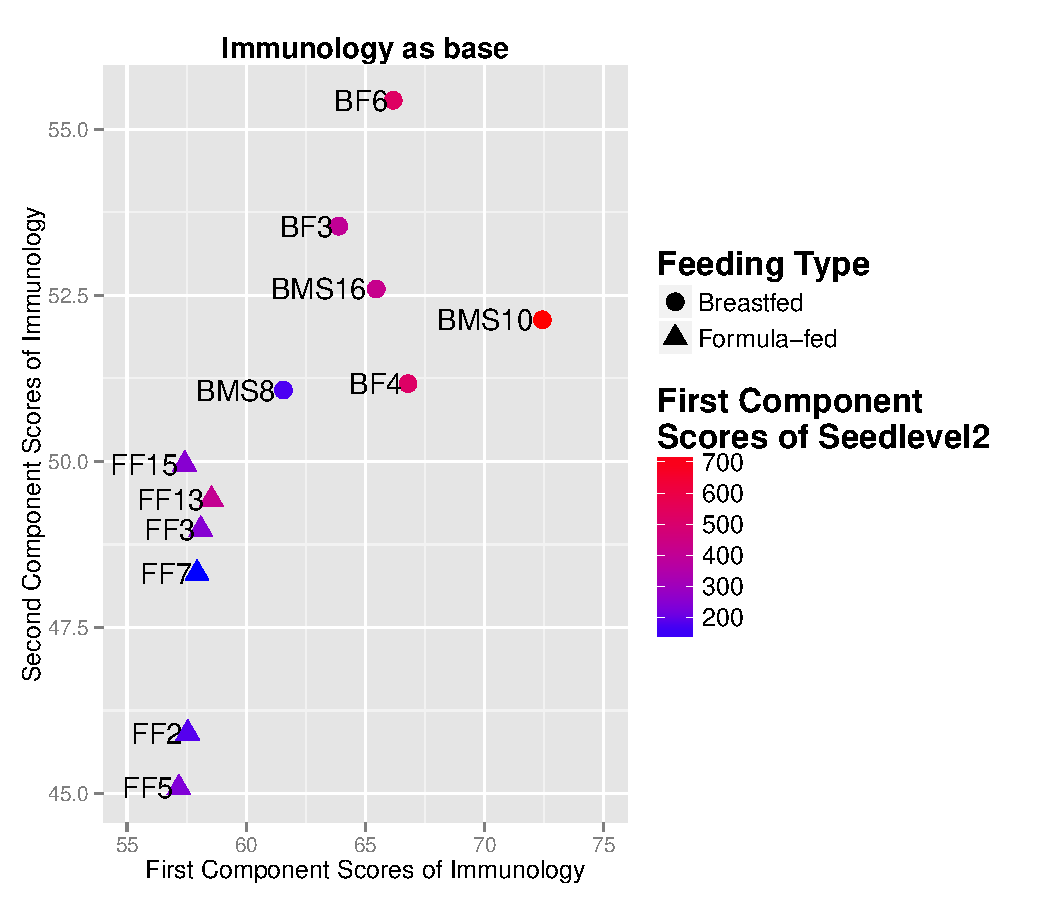
\includegraphics[width=\maxwidth]{figure/Nov_16-2} 

}

\end{Schunk}
 \subsection{Nov 25}
 more ggplot the scaterplots of the components
\begin{Schunk}


{\centering 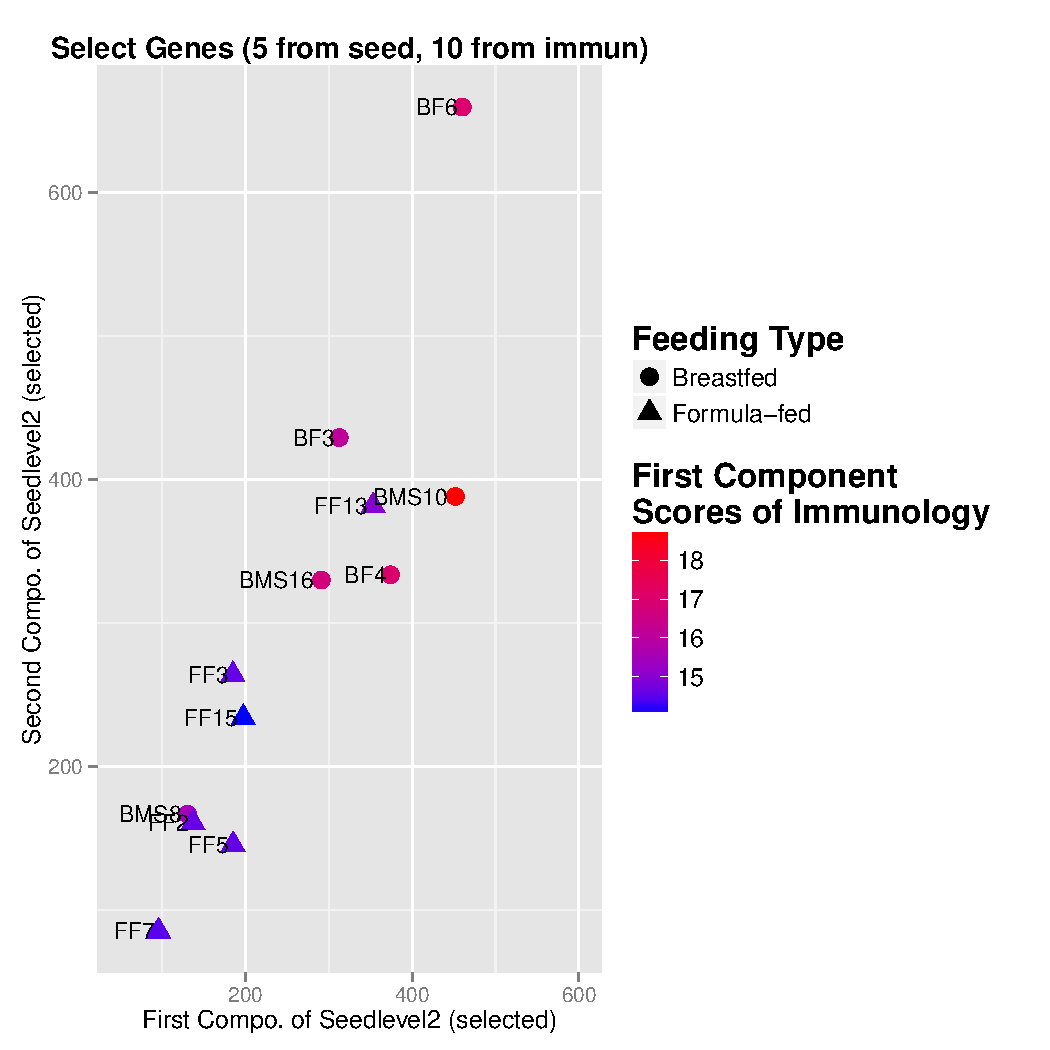
\includegraphics[width=\maxwidth]{figure/Nov_25-1} 

}



{\centering 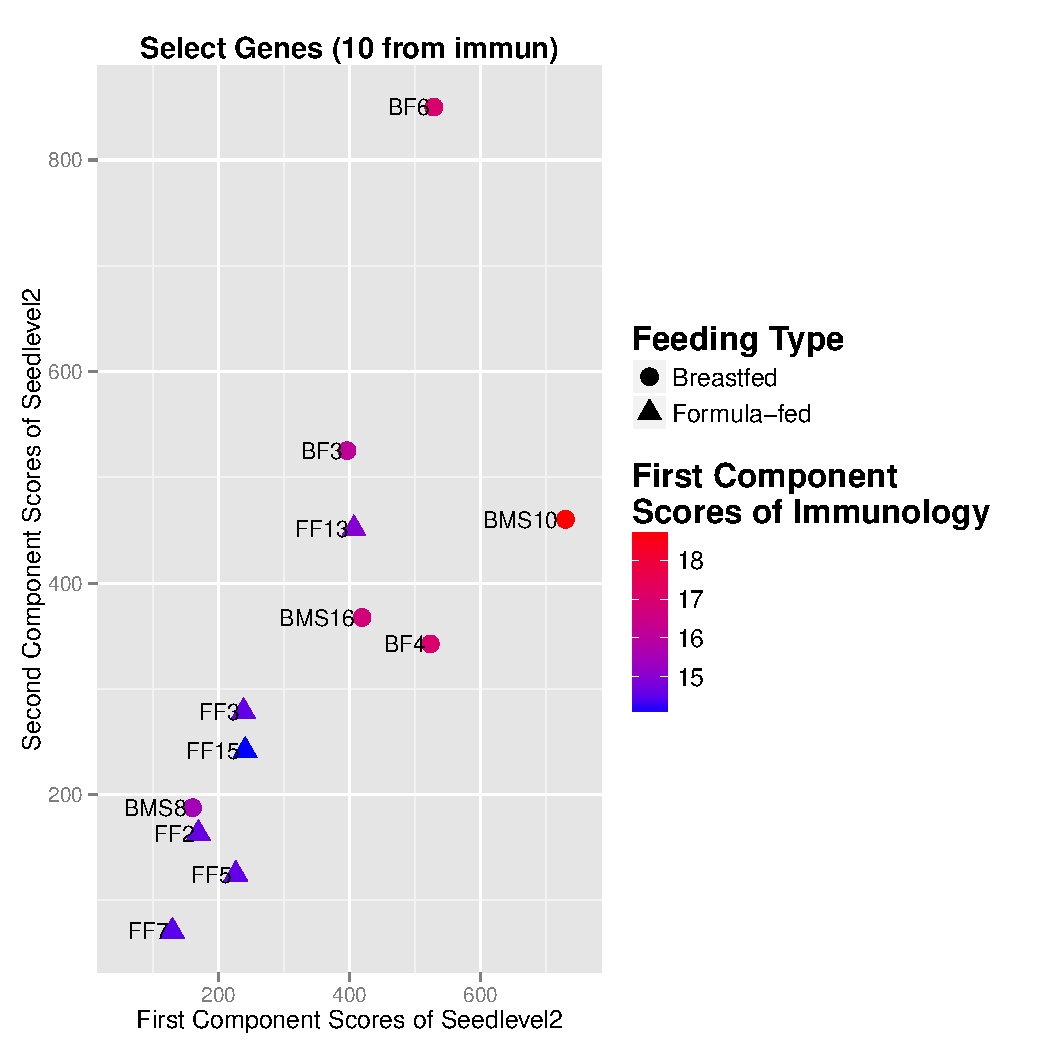
\includegraphics[width=\maxwidth]{figure/Nov_25-2} 

}



{\centering 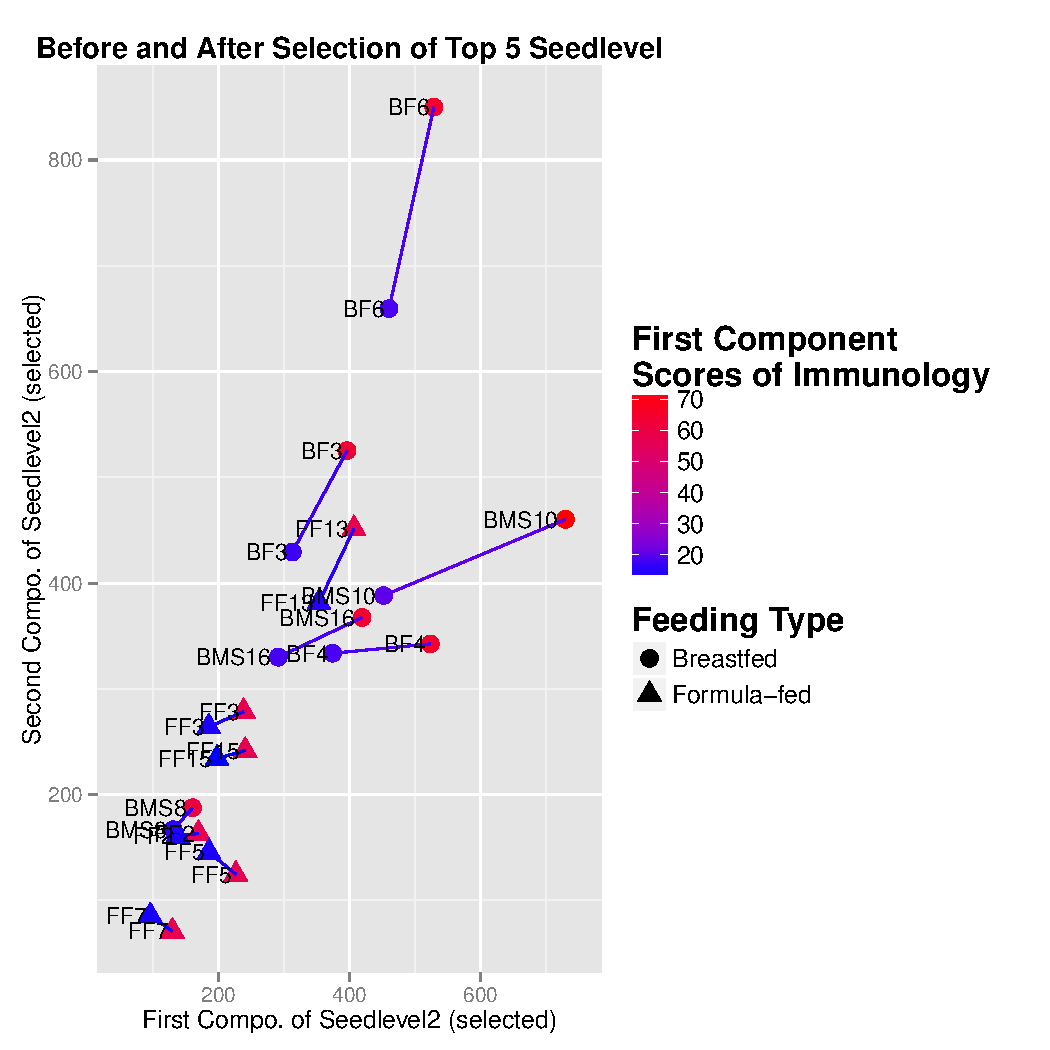
\includegraphics[width=\maxwidth]{figure/Nov_25-3} 

}

\begin{Soutput}
     CD40    SEMA4D     TACR1   HLA-DOB     SNED1      EGFR 
0.2154260 0.2039536 0.1983327 0.1945679 0.1883817 0.1813819 
    CCL18     NOXA1     CCL22     GSTM4 
0.1680291 0.1667387 0.1622053 0.1572842 
      GULP1        TLR4      TBXA2R        LMO2       WNT5A 
 0.00000000  0.00000000  0.00000000  0.00000000  0.00000000 
      FKBP5      SQSTM1         TST      TCF7L2        EGFR 
 0.00000000  0.00000000  0.00000000  0.00000000 -0.07854534 
\end{Soutput}
\end{Schunk}
\end{document}
